\subsection{ArbIS}
\label{analysis_processing_correlation_baysis_matched}
The correlation matrix table for the congestion-roadwork dataset (see \cref{tbl:appendix_arbis_correlation_matrix_dataset_cramers}) is visual presented in \cref{img:correlation_matrix_arbis_selected_effector_cramers} showing the the correlation of each variable combination. When visual analyzing \cref{img:correlation_matrix_arbis_selected_effector_cramers} and checking the guidelines for a strong correlation in reference to the applied coefficient (identifiable with \cref{table:appendix_coefficient_matrix_matched}) we get a list of strongly correlated variable combinations (see \cref{tbl:correlation_list_arbis_matched}). Since the focus of the thesis are the correlations between accidents and jams, these are only collected from the bottom-left rectangle of the matrix, where the congestion and accidents variables intersect.
\begin{table}[h!]
	\centering
	\begin{tabular}{c|l|l}  
		Category & Strong \\
		\\[-1em]
		\hline
		\\[-1em]
		Strasse & TMax, TAvg, SMax, SAvg, TDist, SDist, Cov, TLCar, TLHGV \\ 
 		%AnzGesperrtFs & & \\ 
 		%Einzug & & \\
 		%Richtung & & \\
 		%Length & & \\
 		%Duration & & \\
 		Month & TAvg, SMax, SAvg, TDist, SDist, Cov, TLCar \\
	\end{tabular}
  \caption{List of incident variables and their strong/moderated correlated jam variable from the ArbIS matched data}
  \label{tbl:correlation_list_arbis_matched}
\end{table}
Next we need to verify that the correlation is significant and what the correlation predicates. Therefore each correlation will be evaluated with the Post Hoc test, defined in \cref{correlation_posthoc}. In the following sections, the correlated relations of the variables in \cref{tbl:correlation_list_arbis_matched} are analyzed and an initial interpretation of each significant correlation is introduced. Groups with an insufficient sample size (see \cref{correlation_uncertainty} are neglected and not shown. The descriptive tables, showing the count ($n$), mean ($\bar{x}$), standard deviation ($\sigma$), median ($\tilde{x}$), $min$, $max$ and range ($\Delta$) therefore only contain groups with significant sample sizes.
\begin{figure}[!ht]
	\centering
	\makebox[\textwidth][c]{%
		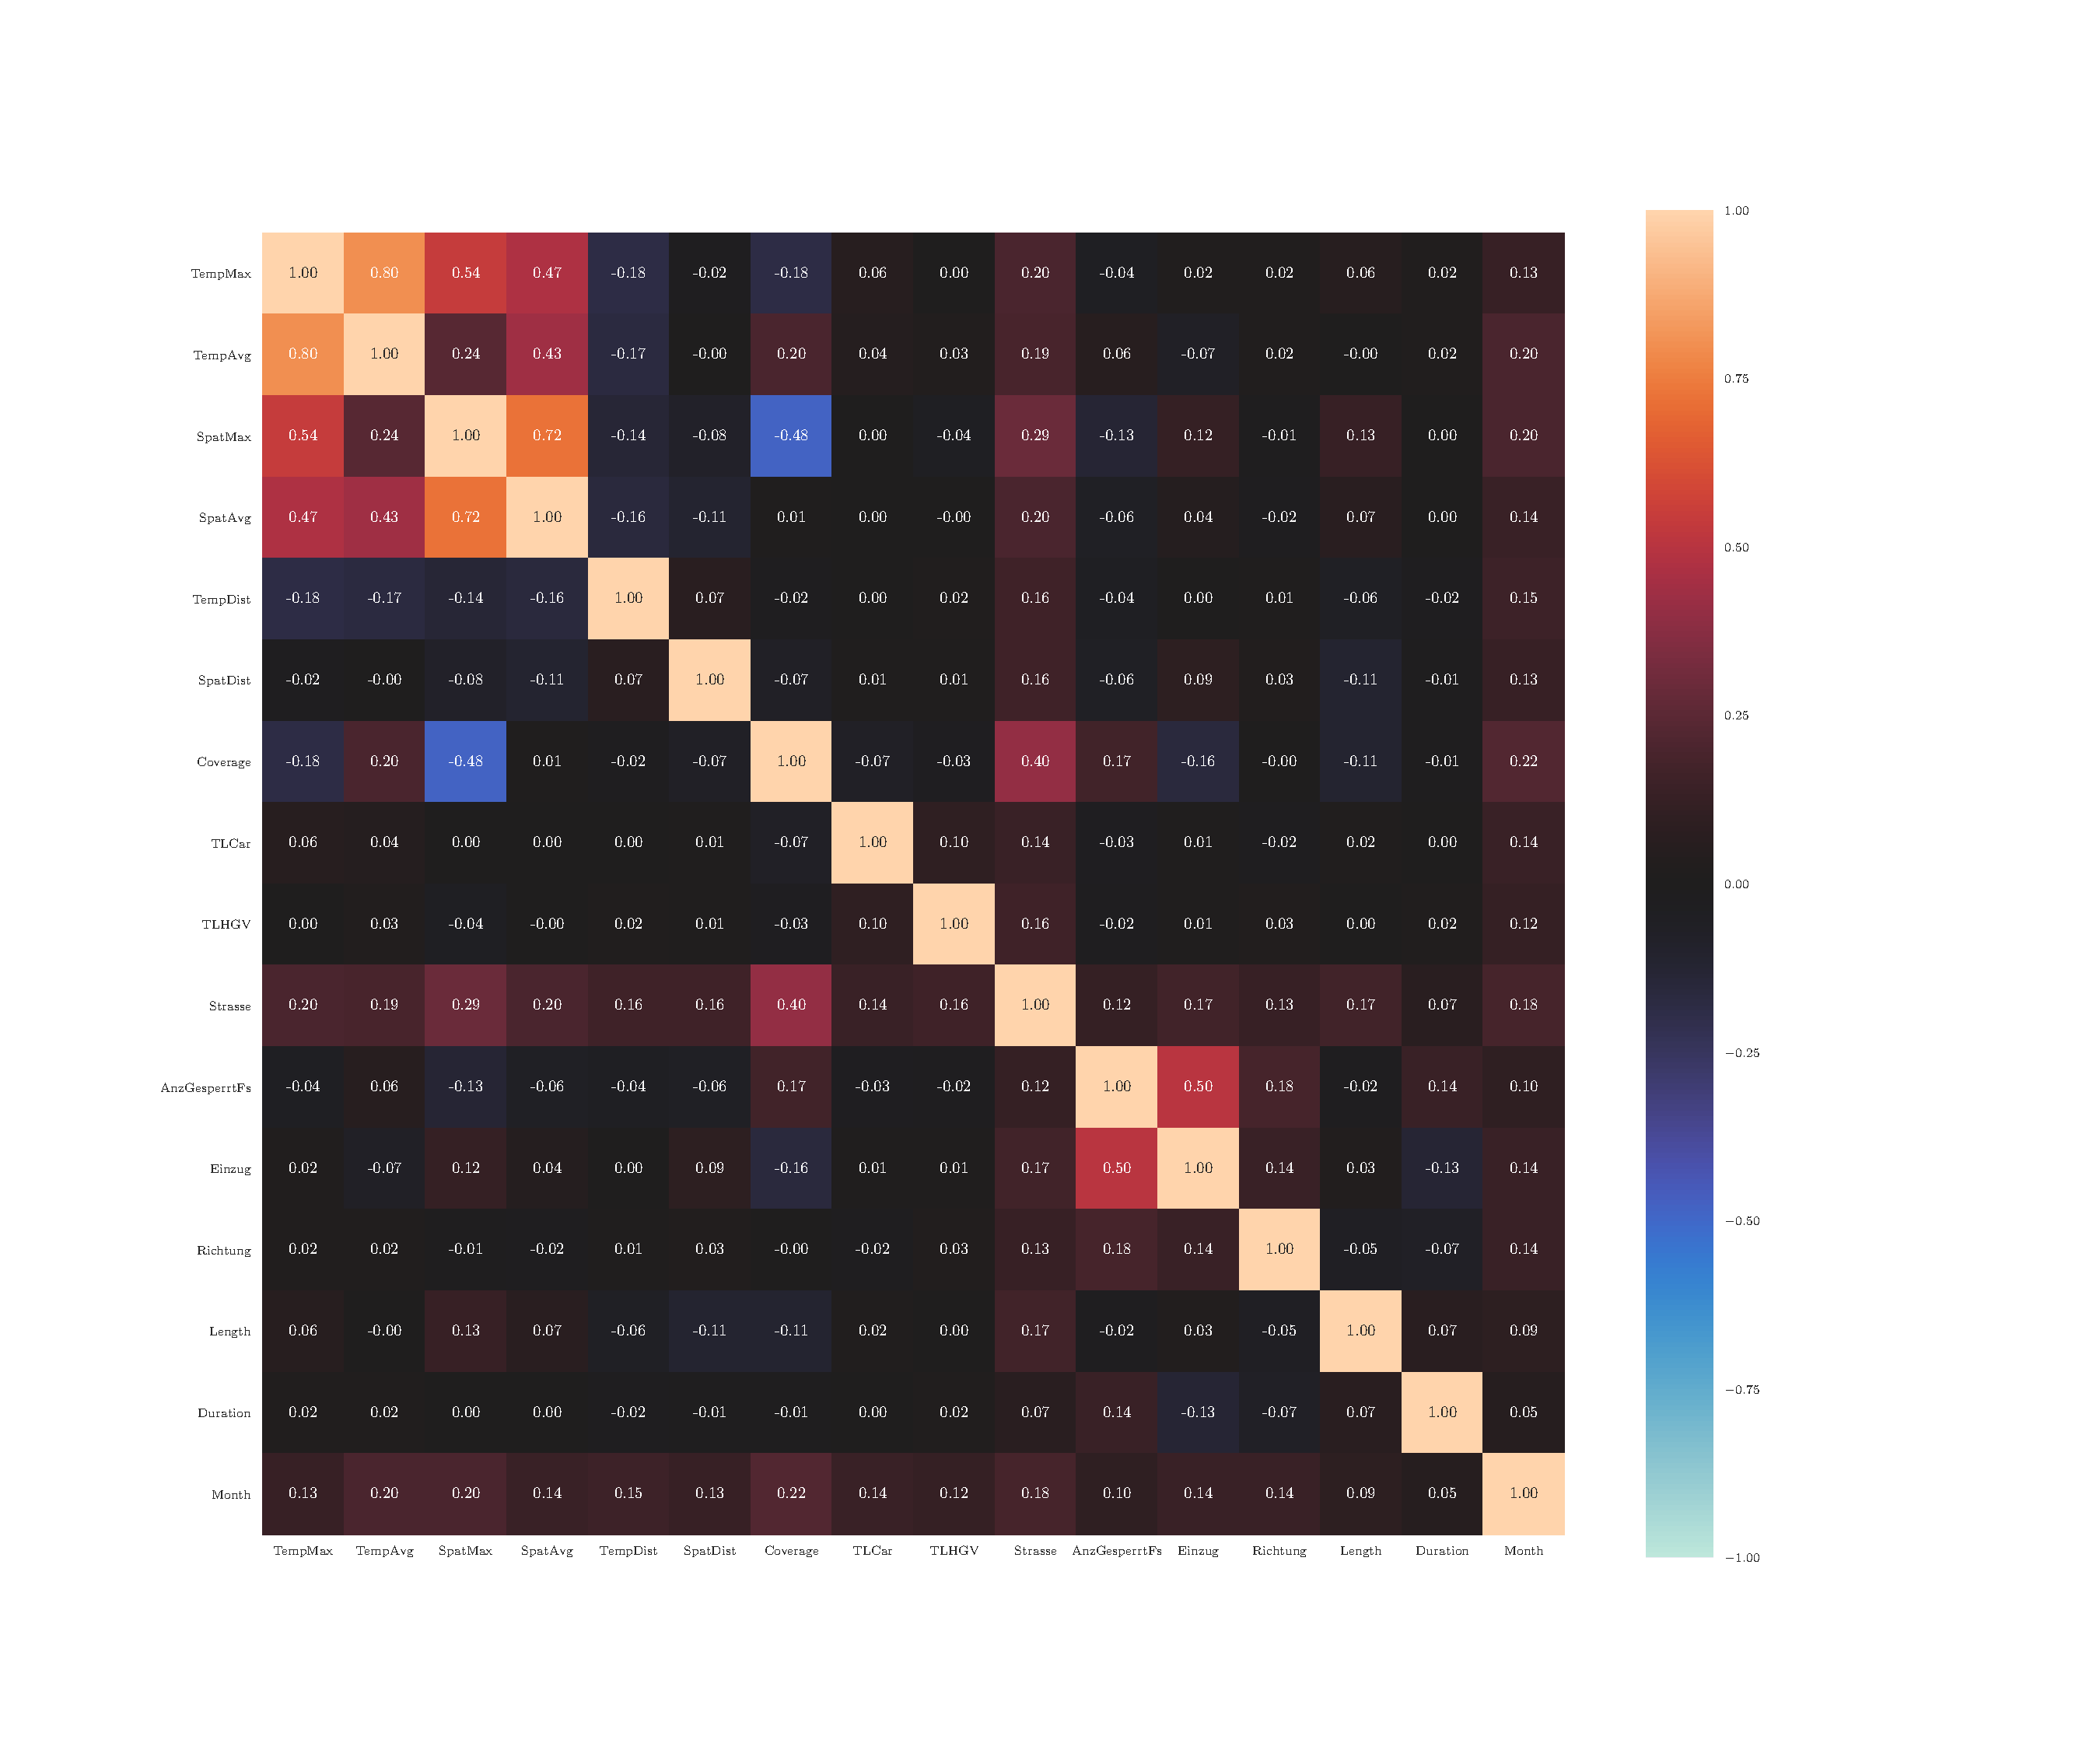
\includegraphics[width=1.4\textwidth, trim=0cm 2.5cm 6cm 3cm]{CorrAnalysis/data/ArbIS/02_matched/plots/arbis_matched_corr_cramers}%
	}
	\caption{Correlation matrix for congestion-roadwork matched data, calculated with $V$, $\eta$, $\tau$, $r_{pq}$, $r$}
	\label{img:correlation_matrix_arbis_selected_effector_cramers}
\end{figure}

% --------------------------
% -------- Strasse ---------
% --------------------------
\centerheading{Strasse}
This section analyzes the correlated relations of the accident variable \textit{Strasse}. The correlations of \textit{Strasse} - \textit{SAvg} and \textit{Strasse} - \textit{TLHGV} produces a $p$-value above the $\alpha$-level of .05 in the Kruskal-Wallis rank sum test. The null hypothesis can't therefore be rejected for these relations and there are no significant groups to identify.

The Kruskal-Wallis rank sum test of \textit{Strasse} - \textit{TMax} produces a $p$-value of 0.003967, which is below $\alpha=.05$. The null hypothesis can therefore be rejected, which means there is a significant difference between the groups of \textit{Strasse}. To identify the significant groups, a pairwise Wilcoxon $T$-test for \textit{Strasse} - \textit{TMax} is run, which produces \cref{tbl:wilcoxon_baysis_effector_Strasse_TMax}. 


\paragraph{Maximal Temporal Extent}
Kruskal-Wallis chi-squared = 957.47, df = 203, p-value < 2.2e-16

\begin{table}[ht!]
	\tiny
	\setlength{\tabcolsep}{4pt}
	\centering
  \begin{tabular}{rrrrrrrrrrrrrrrrr}
    \hline
   & 0 & 1 & 2 & 3 & 4 & 5 & 6 & 7 & 8 & 9 & 10 & 11 & 12 & 13 & 14 & 15 \\ 
    \hline
  1 & 1.00 &  &  &  &  &  &  &  &  &  &  &  &  &  &  &  \\ 
    2 & 1.00 & 1.00 &  &  &  &  &  &  &  &  &  &  &  &  &  &  \\ 
    3 & 1.00 & 1.00 & 1.00 &  &  &  &  &  &  &  &  &  &  &  &  &  \\ 
    4 & 1.00 & 1.00 & 1.00 & 1.00 &  &  &  &  &  &  &  &  &  &  &  &  \\ 
    5 & 1.00 & 1.00 & 1.00 & 1.00 & 1.00 &  &  &  &  &  &  &  &  &  &  &  \\ 
    6 & 0.00 & 0.04 & 1.00 & 1.00 & 0.01 & 1.00 &  &  &  &  &  &  &  &  &  &  \\ 
    7 & 1.00 & 1.00 & 1.00 & 1.00 & 0.48 & 1.00 & 1.00 &  &  &  &  &  &  &  &  &  \\ 
    8 & 1.00 & 0.82 & 1.00 & 1.00 & 1.00 & 1.00 & 0.00 & 0.00 &  &  &  &  &  &  &  &  \\ 
    9 & 1.00 & 1.00 & 1.00 & 1.00 & 1.00 & 1.00 & 0.79 & 0.74 & 1.00 &  &  &  &  &  &  &  \\ 
    10 & 1.00 & 1.00 & 1.00 & 1.00 & 1.00 & 1.00 & 1.00 & 1.00 & 1.00 & 1.00 &  &  &  &  &  &  \\ 
    11 & 1.00 & 1.00 & 1.00 & 1.00 & 1.00 & 1.00 & 1.00 & 1.00 & 1.00 & 1.00 & 1.00 &  &  &  &  &  \\ 
    12 & 0.00 & 0.00 & 1.00 & 0.09 & 0.00 & 0.00 & 1.00 & 1.00 & 0.00 & 0.00 & 0.00 & 1.00 &  &  &  &  \\ 
    13 & 1.00 & 1.00 & 1.00 & 1.00 & 1.00 & 1.00 & 1.00 & 1.00 & 1.00 & 1.00 & 1.00 & 1.00 & 1.00 &  &  &  \\ 
    14 & 1.00 & 1.00 & 1.00 & 1.00 & 0.68 & 1.00 & 1.00 & 1.00 & 0.01 & 0.48 & 1.00 & 1.00 & 1.00 & 1.00 &  &  \\ 
    15 & 1.00 & 1.00 & 1.00 & 1.00 & 1.00 & 1.00 & 1.00 & 1.00 & 1.00 & 1.00 & 1.00 & 1.00 & 1.00 & 1.00 & 1.00 &  \\ 
    16 & 1.00 & 1.00 & 1.00 & 1.00 & 1.00 & 1.00 & 1.00 & 1.00 & 1.00 & 1.00 & 1.00 & 1.00 & 1.00 & 1.00 & 1.00 & 1.00 \\ 
     \hline
  \end{tabular}
	\caption{Pairwise Wilcoxon $T$-test for \textit{Strasse} and \textit{Maximal Temporal Extent}}
	\label{tbl:wilcoxon_baysis_matched_Strasse_TMax}
\end{table}
\cref{tbl:wilcoxon_baysis_matched_Strasse_TMax} shows, that the groups A6, A9, A7, A70, A73, A92, A94 and A96 differ from group A3. There is no distinctive general trend.
\begin{table}[ht!]
	\tiny
	\centering
  \begin{tabular}{rrrrrrrrrrrrrr}
    \hline
   & vars & n & mean & sd & median & trimmed & mad & min & max & range & skew & kurtosis & se \\ 
    \hline
  X1 & 1.00 & 656.00 & 159.55 & 175.78 & 100.50 & 127.02 & 117.87 & 9.00 & 1323.00 & 1314.00 & 2.03 & 5.98 & 6.86 \\ 
    X11 & 1.00 & 302.00 & 158.38 & 213.55 & 87.00 & 111.90 & 77.84 & 9.00 & 1323.00 & 1314.00 & 3.40 & 13.83 & 12.29 \\ 
    X12 & 1.00 & 50.00 & 228.90 & 279.03 & 105.00 & 170.93 & 120.09 & 15.00 & 963.00 & 948.00 & 1.49 & 0.96 & 39.46 \\ 
    X13 & 1.00 & 10.00 & 83.40 & 72.87 & 48.00 & 68.62 & 13.34 & 36.00 & 249.00 & 213.00 & 1.27 & 0.01 & 23.04 \\ 
    X14 & 1.00 & 198.00 & 142.24 & 166.46 & 85.50 & 108.13 & 80.06 & 9.00 & 864.00 & 855.00 & 2.38 & 6.20 & 11.83 \\ 
    X15 & 1.00 & 86.00 & 153.59 & 235.85 & 100.50 & 110.91 & 73.39 & 9.00 & 1323.00 & 1314.00 & 4.21 & 18.12 & 25.43 \\ 
    X16 & 1.00 & 1023.00 & 233.66 & 279.35 & 123.00 & 175.80 & 133.43 & 9.00 & 1326.00 & 1317.00 & 2.03 & 4.20 & 8.73 \\ 
    X17 & 1.00 & 312.00 & 158.88 & 155.05 & 135.00 & 134.74 & 111.19 & 9.00 & 1320.00 & 1311.00 & 3.24 & 18.91 & 8.78 \\ 
    X18 & 1.00 & 230.00 & 105.80 & 95.17 & 75.00 & 90.99 & 71.16 & 9.00 & 384.00 & 375.00 & 1.24 & 0.59 & 6.28 \\ 
    X19 & 1.00 & 14.00 & 60.00 & 28.70 & 48.00 & 59.75 & 42.25 & 18.00 & 105.00 & 87.00 & 0.07 & -1.65 & 7.67 \\ 
    X110 & 1.00 & 82.00 & 132.40 & 134.72 & 79.50 & 109.41 & 77.84 & 9.00 & 768.00 & 759.00 & 2.18 & 6.04 & 14.88 \\ 
    X111 & 1.00 & 3.00 & 425.00 & 313.50 & 606.00 & 425.00 & 0.00 & 63.00 & 606.00 & 543.00 & -0.38 & -2.33 & 181.00 \\ 
    X112 & 1.00 & 160.00 & 157.33 & 55.97 & 189.00 & 164.20 & 17.79 & 9.00 & 312.00 & 303.00 & -0.81 & 0.27 & 4.42 \\ 
    X113 & 1.00 & 2.00 & 117.00 & 106.07 & 117.00 & 117.00 & 111.19 & 42.00 & 192.00 & 150.00 & 0.00 & -2.75 & 75.00 \\ 
    X114 & 1.00 & 56.00 & 179.57 & 124.79 & 165.00 & 175.96 & 180.14 & 15.00 & 369.00 & 354.00 & 0.19 & -1.46 & 16.68 \\ 
    X115 & 1.00 & 3.00 & 83.00 & 27.71 & 99.00 & 83.00 & 0.00 & 51.00 & 99.00 & 48.00 & -0.38 & -2.33 & 16.00 \\ 
    X116 & 1.00 & 2.00 & 123.00 & 0.00 & 123.00 & 123.00 & 0.00 & 123.00 & 123.00 & 0.00 &  &  & 0.00 \\ 
     \hline
  \end{tabular}
	\caption{Group descriptives of \textit{Strasse} and \textit{Maximal Temporal Extent}}
	\label{tbl:descriptives_baysis_matched_Strasse_TMax}
	%\vspace{-8mm}
\end{table}


\paragraph{Average Temporal Extent}
Kruskal-Wallis chi-squared = 1050.6, df = 256, p-value < 2.2e-16

\begin{table}[ht!]
	\tiny
	\setlength{\tabcolsep}{4pt}
	\centering
  \begin{tabular}{rrrrrrrrrrrrrrrrr}
    \hline
   & 0 & 1 & 2 & 3 & 4 & 5 & 6 & 7 & 8 & 9 & 10 & 11 & 12 & 13 & 14 & 15 \\ 
    \hline
  1 & 1.00 &  &  &  &  &  &  &  &  &  &  &  &  &  &  &  \\ 
    2 & 1.00 & 1.00 &  &  &  &  &  &  &  &  &  &  &  &  &  &  \\ 
    3 & 1.00 & 1.00 & 1.00 &  &  &  &  &  &  &  &  &  &  &  &  &  \\ 
    4 & 1.00 & 1.00 & 1.00 & 1.00 &  &  &  &  &  &  &  &  &  &  &  &  \\ 
    5 & 1.00 & 1.00 & 1.00 & 1.00 & 1.00 &  &  &  &  &  &  &  &  &  &  &  \\ 
    6 & 1.00 & 1.00 & 1.00 & 1.00 & 0.69 & 1.00 &  &  &  &  &  &  &  &  &  &  \\ 
    7 & 0.00 & 0.00 & 0.08 & 1.00 & 1.00 & 1.00 & 0.00 &  &  &  &  &  &  &  &  &  \\ 
    8 & 1.00 & 1.00 & 1.00 & 1.00 & 1.00 & 1.00 & 1.00 & 0.55 &  &  &  &  &  &  &  &  \\ 
    9 & 1.00 & 1.00 & 1.00 & 1.00 & 1.00 & 1.00 & 1.00 & 1.00 & 1.00 &  &  &  &  &  &  &  \\ 
    10 & 1.00 & 1.00 & 1.00 & 1.00 & 1.00 & 1.00 & 1.00 & 0.04 & 1.00 & 1.00 &  &  &  &  &  &  \\ 
    11 & 1.00 & 1.00 & 1.00 & 1.00 & 1.00 & 1.00 & 1.00 & 1.00 & 1.00 & 1.00 & 1.00 &  &  &  &  &  \\ 
    12 & 0.00 & 0.00 & 1.00 & 0.24 & 0.00 & 0.00 & 0.00 & 0.00 & 0.00 & 0.00 & 0.00 & 1.00 &  &  &  &  \\ 
    13 & 1.00 & 1.00 & 1.00 & 1.00 & 1.00 & 1.00 & 1.00 & 1.00 & 1.00 & 1.00 & 1.00 & 1.00 & 1.00 &  &  &  \\ 
    14 & 1.00 & 1.00 & 1.00 & 1.00 & 0.14 & 1.00 & 1.00 & 0.00 & 0.63 & 0.53 & 1.00 & 1.00 & 0.02 & 1.00 &  &  \\ 
    15 & 1.00 & 1.00 & 1.00 & 1.00 & 1.00 & 1.00 & 1.00 & 1.00 & 1.00 & 1.00 & 1.00 & 1.00 & 1.00 & 1.00 & 1.00 &  \\ 
    16 & 1.00 & 1.00 & 1.00 & 1.00 & 1.00 & 1.00 & 1.00 & 1.00 & 1.00 & 1.00 & 1.00 & 1.00 & 1.00 & 1.00 & 1.00 & 1.00 \\ 
     \hline
  \end{tabular}
	\caption{Pairwise Wilcoxon $T$-test for \textit{Strasse} and \textit{Maximal Temporal Extent}}
	\label{tbl:wilcoxon_baysis_matched_Strasse_TMax}
\end{table}
\cref{tbl:wilcoxon_baysis_matched_Strasse_TMax} shows, that the groups A6, A9, A7, A70, A73, A92, A94 and A96 differ from group A3. There is no distinctive general trend.
\begin{table}[ht!]
	\tiny
	\centering
  \begin{tabular}{rrrrrrrrrrrrrr}
    \hline
   & vars & n & mean & sd & median & trimmed & mad & min & max & range & skew & kurtosis & se \\ 
    \hline
  X1 & 1.00 & 656.00 & 85.61 & 100.78 & 42.00 & 64.66 & 41.51 & 5.00 & 575.00 & 570.00 & 2.12 & 4.76 & 3.93 \\ 
    X11 & 1.00 & 302.00 & 87.76 & 117.13 & 44.50 & 60.64 & 40.77 & 5.00 & 858.00 & 853.00 & 3.03 & 12.53 & 6.74 \\ 
    X12 & 1.00 & 50.00 & 154.38 & 236.49 & 55.50 & 93.28 & 52.63 & 6.00 & 966.00 & 960.00 & 2.20 & 4.03 & 33.44 \\ 
    X13 & 1.00 & 10.00 & 64.90 & 71.81 & 38.00 & 47.38 & 21.50 & 18.00 & 252.00 & 234.00 & 1.72 & 1.69 & 22.71 \\ 
    X14 & 1.00 & 198.00 & 65.60 & 86.36 & 41.00 & 47.58 & 38.55 & 4.00 & 630.00 & 626.00 & 3.44 & 14.50 & 6.14 \\ 
    X15 & 1.00 & 86.00 & 56.23 & 45.35 & 42.50 & 50.14 & 31.88 & 6.00 & 190.00 & 184.00 & 1.14 & 0.32 & 4.89 \\ 
    X16 & 1.00 & 1023.00 & 89.94 & 124.69 & 51.00 & 64.57 & 54.86 & 3.00 & 1326.00 & 1323.00 & 4.52 & 32.41 & 3.90 \\ 
    X17 & 1.00 & 312.00 & 45.38 & 41.73 & 33.00 & 37.99 & 25.20 & 3.00 & 291.00 & 288.00 & 2.30 & 7.77 & 2.36 \\ 
    X18 & 1.00 & 230.00 & 69.31 & 73.52 & 43.00 & 53.59 & 39.29 & 5.00 & 290.00 & 285.00 & 1.64 & 1.70 & 4.85 \\ 
    X19 & 1.00 & 14.00 & 37.14 & 23.98 & 23.00 & 36.50 & 20.02 & 8.00 & 74.00 & 66.00 & 0.23 & -1.87 & 6.41 \\ 
    X110 & 1.00 & 82.00 & 81.83 & 90.35 & 45.50 & 65.23 & 40.77 & 5.00 & 489.00 & 484.00 & 2.24 & 5.95 & 9.98 \\ 
    X111 & 1.00 & 3.00 & 333.67 & 267.31 & 488.00 & 333.67 & 0.00 & 25.00 & 488.00 & 463.00 & -0.38 & -2.33 & 154.33 \\ 
    X112 & 1.00 & 160.00 & 115.96 & 50.96 & 141.00 & 121.91 & 31.13 & 6.00 & 199.00 & 193.00 & -0.62 & -1.03 & 4.03 \\ 
    X113 & 1.00 & 2.00 & 60.50 & 23.33 & 60.50 & 60.50 & 24.46 & 44.00 & 77.00 & 33.00 & 0.00 & -2.75 & 16.50 \\ 
    X114 & 1.00 & 56.00 & 84.98 & 64.07 & 70.00 & 77.70 & 65.98 & 6.00 & 248.00 & 242.00 & 0.84 & -0.12 & 8.56 \\ 
    X115 & 1.00 & 3.00 & 62.33 & 34.06 & 82.00 & 62.33 & 0.00 & 23.00 & 82.00 & 59.00 & -0.38 & -2.33 & 19.67 \\ 
    X116 & 1.00 & 2.00 & 107.00 & 0.00 & 107.00 & 107.00 & 0.00 & 107.00 & 107.00 & 0.00 &  &  & 0.00 \\ 
     \hline
  \end{tabular}
	\caption{Group descriptives of \textit{Strasse} and \textit{Maximal Temporal Extent}}
	\label{tbl:descriptives_baysis_matched_Strasse_TMax}
	%\vspace{-8mm}
\end{table}

\paragraph{Maximal Spatial Extent}
Kruskal-Wallis chi-squared = 3082.1, df = 1228, p-value < 2.2e-16

\begin{table}[ht!]
	\tiny
	\setlength{\tabcolsep}{4pt}
	\centering
  \begin{tabular}{rrrrrrrrrrrrrrrrr}
    \hline
   & 0 & 1 & 2 & 3 & 4 & 5 & 6 & 7 & 8 & 9 & 10 & 11 & 12 & 13 & 14 & 15 \\ 
    \hline
  1 & 0.58 &  &  &  &  &  &  &  &  &  &  &  &  &  &  &  \\ 
    2 & 1.00 & 1.00 &  &  &  &  &  &  &  &  &  &  &  &  &  &  \\ 
    3 & 1.00 & 1.00 & 1.00 &  &  &  &  &  &  &  &  &  &  &  &  &  \\ 
    4 & 1.00 & 1.00 & 1.00 & 1.00 &  &  &  &  &  &  &  &  &  &  &  &  \\ 
    5 & 1.00 & 1.00 & 1.00 & 1.00 & 1.00 &  &  &  &  &  &  &  &  &  &  &  \\ 
    6 & 0.00 & 0.00 & 0.00 & 0.52 & 0.01 & 0.05 &  &  &  &  &  &  &  &  &  &  \\ 
    7 & 0.07 & 0.00 & 0.01 & 0.21 & 0.26 & 0.20 & 1.00 &  &  &  &  &  &  &  &  &  \\ 
    8 & 0.00 & 0.06 & 1.00 & 1.00 & 0.00 & 1.00 & 0.00 & 0.00 &  &  &  &  &  &  &  &  \\ 
    9 & 1.00 & 1.00 & 1.00 & 1.00 & 1.00 & 1.00 & 0.11 & 0.03 & 1.00 &  &  &  &  &  &  &  \\ 
    10 & 1.00 & 1.00 & 1.00 & 1.00 & 1.00 & 1.00 & 0.00 & 0.00 & 0.04 & 1.00 &  &  &  &  &  &  \\ 
    11 & 1.00 & 1.00 & 1.00 & 1.00 & 1.00 & 1.00 & 1.00 & 1.00 & 1.00 & 0.81 & 1.00 &  &  &  &  &  \\ 
    12 & 0.00 & 0.00 & 0.02 & 1.00 & 0.00 & 0.00 & 0.00 & 0.00 & 0.00 & 1.00 & 0.00 & 0.73 &  &  &  &  \\ 
    13 & 1.00 & 1.00 & 1.00 & 1.00 & 1.00 & 1.00 & 1.00 & 1.00 & 1.00 & 1.00 & 1.00 & 1.00 & 1.00 &  &  &  \\ 
    14 & 1.00 & 1.00 & 1.00 & 1.00 & 1.00 & 1.00 & 0.04 & 0.04 & 0.89 & 1.00 & 1.00 & 1.00 & 0.00 & 1.00 &  &  \\ 
    15 & 1.00 & 1.00 & 1.00 & 1.00 & 1.00 & 1.00 & 1.00 & 1.00 & 1.00 & 1.00 & 1.00 & 1.00 & 1.00 & 1.00 & 1.00 &  \\ 
    16 & 1.00 & 1.00 & 1.00 & 1.00 & 1.00 & 1.00 & 1.00 & 1.00 & 1.00 & 1.00 & 1.00 & 1.00 & 1.00 & 1.00 & 1.00 & 1.00 \\ 
     \hline
  \end{tabular}
	\caption{Pairwise Wilcoxon $T$-test for \textit{Strasse} and \textit{Maximal Temporal Extent}}
	\label{tbl:wilcoxon_baysis_matched_Strasse_TMax}
\end{table}
\cref{tbl:wilcoxon_baysis_matched_Strasse_TMax} shows, that the groups A6, A9, A7, A70, A73, A92, A94 and A96 differ from group A3. There is no distinctive general trend.
\begin{table}[ht!]
	\tiny
	\centering
  \begin{tabular}{rrrrrrrrrrrrrr}
    \hline
   & vars & n & mean & sd & median & trimmed & mad & min & max & range & skew & kurtosis & se \\ 
    \hline
  X1 & 1.00 & 656.00 & 8655.57 & 8521.51 & 4778.00 & 6972.99 & 3783.60 & 1035.00 & 49765.00 & 48730.00 & 1.85 & 3.49 & 332.71 \\ 
    X11 & 1.00 & 302.00 & 6238.63 & 4902.30 & 4397.00 & 5486.83 & 2874.76 & 902.00 & 20030.00 & 19128.00 & 1.21 & 0.37 & 282.10 \\ 
    X12 & 1.00 & 50.00 & 5729.56 & 4763.20 & 3224.00 & 4856.50 & 2511.52 & 1365.00 & 20249.00 & 18884.00 & 1.39 & 1.03 & 673.62 \\ 
    X13 & 1.00 & 10.00 & 3899.00 & 2746.84 & 2339.00 & 3336.25 & 391.41 & 2075.00 & 10225.00 & 8150.00 & 1.20 & 0.06 & 868.63 \\ 
    X14 & 1.00 & 198.00 & 8421.67 & 8209.85 & 5690.00 & 6919.39 & 4487.83 & 965.00 & 40033.00 & 39068.00 & 1.83 & 3.14 & 583.45 \\ 
    X15 & 1.00 & 86.00 & 7717.21 & 7747.18 & 4813.00 & 6183.17 & 4233.56 & 1095.00 & 33764.00 & 32669.00 & 1.99 & 3.84 & 835.40 \\ 
    X16 & 1.00 & 1023.00 & 11836.50 & 11045.29 & 7979.00 & 9944.23 & 7856.30 & 1014.00 & 47607.00 & 46593.00 & 1.40 & 1.38 & 345.33 \\ 
    X17 & 1.00 & 312.00 & 9337.49 & 7230.99 & 7978.00 & 8264.88 & 6980.82 & 991.00 & 48987.00 & 47996.00 & 1.78 & 4.68 & 409.37 \\ 
    X18 & 1.00 & 230.00 & 5639.41 & 6034.92 & 3072.00 & 4226.37 & 1856.96 & 951.00 & 27965.00 & 27014.00 & 2.07 & 3.48 & 397.93 \\ 
    X19 & 1.00 & 14.00 & 3618.14 & 1331.10 & 4288.00 & 3684.67 & 796.16 & 1613.00 & 4825.00 & 3212.00 & -0.35 & -1.78 & 355.75 \\ 
    X110 & 1.00 & 82.00 & 5758.10 & 3673.73 & 4544.00 & 5227.71 & 3114.94 & 999.00 & 16931.00 & 15932.00 & 1.22 & 0.92 & 405.70 \\ 
    X111 & 1.00 & 3.00 & 8253.67 & 506.34 & 8546.00 & 8253.67 & 0.00 & 7669.00 & 8546.00 & 877.00 & -0.38 & -2.33 & 292.33 \\ 
    X112 & 1.00 & 160.00 & 3530.39 & 3718.54 & 1926.00 & 2571.59 & 34.10 & 699.00 & 22528.00 & 21829.00 & 3.21 & 9.95 & 293.98 \\ 
    X113 & 1.00 & 2.00 & 4020.00 & 4133.75 & 4020.00 & 4020.00 & 4333.64 & 1097.00 & 6943.00 & 5846.00 & 0.00 & -2.75 & 2923.00 \\ 
    X114 & 1.00 & 56.00 & 5849.05 & 3394.57 & 5785.00 & 5667.57 & 2513.01 & 1025.00 & 12582.00 & 11557.00 & 0.47 & -0.67 & 453.62 \\ 
    X115 & 1.00 & 3.00 & 2791.33 & 1500.53 & 1925.00 & 2791.33 & 0.00 & 1925.00 & 4524.00 & 2599.00 & 0.38 & -2.33 & 866.33 \\ 
    X116 & 1.00 & 2.00 & 2075.00 & 0.00 & 2075.00 & 2075.00 & 0.00 & 2075.00 & 2075.00 & 0.00 &  &  & 0.00 \\ 
     \hline
  \end{tabular}
	\caption{Group descriptives of \textit{Strasse} and \textit{Maximal Temporal Extent}}
	\label{tbl:descriptives_baysis_matched_Strasse_TMax}
	%\vspace{-8mm}
\end{table}

\paragraph{Average Spatial Extent}
Kruskal-Wallis chi-squared = 2889, df = 1319, p-value < 2.2e-16

\begin{table}[ht!]
	\tiny
	\setlength{\tabcolsep}{4pt}
	\centering
  \begin{tabular}{rrrrrrrrrrrrrrrrr}
    \hline
   & 0 & 1 & 2 & 3 & 4 & 5 & 6 & 7 & 8 & 9 & 10 & 11 & 12 & 13 & 14 & 15 \\ 
    \hline
  1 & 0.06 &  &  &  &  &  &  &  &  &  &  &  &  &  &  &  \\ 
    2 & 1.00 & 1.00 &  &  &  &  &  &  &  &  &  &  &  &  &  &  \\ 
    3 & 1.00 & 1.00 & 1.00 &  &  &  &  &  &  &  &  &  &  &  &  &  \\ 
    4 & 1.00 & 1.00 & 1.00 & 1.00 &  &  &  &  &  &  &  &  &  &  &  &  \\ 
    5 & 0.62 & 1.00 & 1.00 & 1.00 & 1.00 &  &  &  &  &  &  &  &  &  &  &  \\ 
    6 & 1.00 & 0.00 & 1.00 & 1.00 & 1.00 & 0.02 &  &  &  &  &  &  &  &  &  &  \\ 
    7 & 0.01 & 1.00 & 1.00 & 1.00 & 0.75 & 1.00 & 0.00 &  &  &  &  &  &  &  &  &  \\ 
    8 & 0.00 & 1.00 & 1.00 & 1.00 & 0.44 & 1.00 & 0.00 & 1.00 &  &  &  &  &  &  &  &  \\ 
    9 & 1.00 & 1.00 & 1.00 & 1.00 & 1.00 & 1.00 & 1.00 & 1.00 & 1.00 &  &  &  &  &  &  &  \\ 
    10 & 1.00 & 0.62 & 1.00 & 1.00 & 1.00 & 0.73 & 1.00 & 0.10 & 0.14 & 1.00 &  &  &  &  &  &  \\ 
    11 & 1.00 & 1.00 & 1.00 & 1.00 & 1.00 & 1.00 & 1.00 & 1.00 & 1.00 & 1.00 & 1.00 &  &  &  &  &  \\ 
    12 & 0.00 & 0.13 & 1.00 & 1.00 & 0.00 & 1.00 & 0.00 & 0.11 & 1.00 & 1.00 & 0.00 & 1.00 &  &  &  &  \\ 
    13 & 1.00 & 1.00 & 1.00 & 1.00 & 1.00 & 1.00 & 1.00 & 1.00 & 1.00 & 1.00 & 1.00 & 1.00 & 1.00 &  &  &  \\ 
    14 & 1.00 & 1.00 & 1.00 & 1.00 & 1.00 & 1.00 & 1.00 & 1.00 & 1.00 & 1.00 & 1.00 & 1.00 & 1.00 & 1.00 &  &  \\ 
    15 & 1.00 & 1.00 & 1.00 & 1.00 & 1.00 & 1.00 & 1.00 & 1.00 & 1.00 & 1.00 & 1.00 & 1.00 & 1.00 & 1.00 & 1.00 &  \\ 
    16 & 1.00 & 1.00 & 1.00 & 1.00 & 1.00 & 1.00 & 1.00 & 1.00 & 1.00 & 1.00 & 1.00 & 1.00 & 1.00 & 1.00 & 1.00 & 1.00 \\ 
     \hline
  \end{tabular}
	\caption{Pairwise Wilcoxon $T$-test for \textit{Strasse} and \textit{Maximal Temporal Extent}}
	\label{tbl:wilcoxon_baysis_matched_Strasse_TMax}
\end{table}
\cref{tbl:wilcoxon_baysis_matched_Strasse_TMax} shows, that the groups A6, A9, A7, A70, A73, A92, A94 and A96 differ from group A3. There is no distinctive general trend.
\begin{table}[ht!]
	\tiny
	\centering
  \begin{tabular}{rrrrrrrrrrrrrr}
    \hline
   & vars & n & mean & sd & median & trimmed & mad & min & max & range & skew & kurtosis & se \\ 
    \hline
  X1 & 1.00 & 656.00 & 3537.87 & 3014.80 & 2388.50 & 2920.30 & 1381.78 & 697.00 & 14785.00 & 14088.00 & 1.76 & 2.51 & 117.71 \\ 
    X11 & 1.00 & 302.00 & 2917.97 & 2988.99 & 2113.50 & 2271.17 & 1127.52 & 284.00 & 15602.00 & 15318.00 & 3.08 & 9.64 & 172.00 \\ 
    X12 & 1.00 & 50.00 & 3170.10 & 3033.98 & 1816.00 & 2516.70 & 962.21 & 532.00 & 12543.00 & 12011.00 & 1.72 & 1.88 & 429.07 \\ 
    X13 & 1.00 & 10.00 & 2572.50 & 3027.05 & 1323.00 & 1812.25 & 690.89 & 802.00 & 10425.00 & 9623.00 & 1.73 & 1.62 & 957.24 \\ 
    X14 & 1.00 & 198.00 & 3189.79 & 2385.78 & 2267.00 & 2780.79 & 1272.07 & 458.00 & 14150.00 & 13692.00 & 1.63 & 2.60 & 169.55 \\ 
    X15 & 1.00 & 86.00 & 2508.40 & 1834.03 & 2006.00 & 2228.70 & 1316.55 & 419.00 & 10039.00 & 9620.00 & 1.86 & 4.15 & 197.77 \\ 
    X16 & 1.00 & 1023.00 & 3733.90 & 2979.43 & 2835.00 & 3227.67 & 2269.86 & 355.00 & 15054.00 & 14699.00 & 1.54 & 2.09 & 93.15 \\ 
    X17 & 1.00 & 312.00 & 2381.29 & 1265.40 & 1974.00 & 2225.76 & 1073.40 & 502.00 & 5931.00 & 5429.00 & 1.00 & 0.27 & 71.64 \\ 
    X18 & 1.00 & 230.00 & 2488.22 & 1790.94 & 2160.00 & 2144.86 & 1068.21 & 404.00 & 9767.00 & 9363.00 & 2.10 & 4.77 & 118.09 \\ 
    X19 & 1.00 & 14.00 & 1976.93 & 1044.51 & 1950.00 & 1992.67 & 1714.63 & 569.00 & 3196.00 & 2627.00 & 0.06 & -1.72 & 279.16 \\ 
    X110 & 1.00 & 82.00 & 3360.88 & 2294.30 & 2882.00 & 3040.65 & 1786.53 & 457.00 & 11703.00 & 11246.00 & 1.27 & 1.23 & 253.36 \\ 
    X111 & 1.00 & 3.00 & 3808.67 & 1292.69 & 4555.00 & 3808.67 & 0.00 & 2316.00 & 4555.00 & 2239.00 & -0.38 & -2.33 & 746.33 \\ 
    X112 & 1.00 & 160.00 & 2243.26 & 2065.34 & 1575.00 & 1749.74 & 449.23 & 461.00 & 11161.00 & 10700.00 & 3.42 & 11.30 & 163.28 \\ 
    X113 & 1.00 & 2.00 & 2093.50 & 1584.63 & 2093.50 & 2093.50 & 1661.25 & 973.00 & 3214.00 & 2241.00 & 0.00 & -2.75 & 1120.50 \\ 
    X114 & 1.00 & 56.00 & 2557.62 & 1655.86 & 2551.00 & 2354.04 & 1104.54 & 506.00 & 6393.00 & 5887.00 & 1.06 & 0.54 & 221.27 \\ 
    X115 & 1.00 & 3.00 & 1835.00 & 315.23 & 1653.00 & 1835.00 & 0.00 & 1653.00 & 2199.00 & 546.00 & 0.38 & -2.33 & 182.00 \\ 
    X116 & 1.00 & 2.00 & 1884.00 & 0.00 & 1884.00 & 1884.00 & 0.00 & 1884.00 & 1884.00 & 0.00 &  &  & 0.00 \\ 
     \hline
  \end{tabular}
	\caption{Group descriptives of \textit{Strasse} and \textit{Maximal Temporal Extent}}
	\label{tbl:descriptives_baysis_matched_Strasse_TMax}
	%\vspace{-8mm}
\end{table}

\paragraph{Temporal Distance}
Kruskal-Wallis chi-squared = 58.971, df = 24, p-value = 8.911e-05

\begin{table}[ht!]
	\tiny
	\setlength{\tabcolsep}{4pt}
	\centering
  \begin{tabular}{rrrrrrrrrrrrrrrrr}
    \hline
   & 0 & 1 & 2 & 3 & 4 & 5 & 6 & 7 & 8 & 9 & 10 & 11 & 12 & 13 & 14 & 15 \\ 
    \hline
  1 & 0.00 &  &  &  &  &  &  &  &  &  &  &  &  &  &  &  \\ 
    2 & 0.57 & 1.00 &  &  &  &  &  &  &  &  &  &  &  &  &  &  \\ 
    3 & 1.00 & 1.00 & 1.00 &  &  &  &  &  &  &  &  &  &  &  &  &  \\ 
    4 & 0.10 & 1.00 & 1.00 & 1.00 &  &  &  &  &  &  &  &  &  &  &  &  \\ 
    5 & 1.00 & 1.00 & 1.00 & 1.00 & 1.00 &  &  &  &  &  &  &  &  &  &  &  \\ 
    6 & 0.00 & 1.00 & 1.00 & 1.00 & 1.00 & 0.85 &  &  &  &  &  &  &  &  &  &  \\ 
    7 & 0.38 & 1.00 & 1.00 & 1.00 & 1.00 & 1.00 & 0.26 &  &  &  &  &  &  &  &  &  \\ 
    8 & 1.00 & 1.00 & 1.00 & 1.00 & 1.00 & 1.00 & 0.03 & 1.00 &  &  &  &  &  &  &  &  \\ 
    9 & 1.00 & 1.00 & 1.00 & 1.00 & 1.00 & 1.00 & 1.00 & 1.00 & 1.00 &  &  &  &  &  &  &  \\ 
    10 & 0.04 & 1.00 & 1.00 & 1.00 & 1.00 & 1.00 & 1.00 & 1.00 & 1.00 & 1.00 &  &  &  &  &  &  \\ 
    11 & 1.00 & 1.00 & 1.00 & 1.00 & 1.00 & 1.00 & 1.00 & 1.00 & 1.00 & 1.00 & 1.00 &  &  &  &  &  \\ 
    12 & 0.63 & 1.00 & 1.00 & 1.00 & 1.00 & 1.00 & 1.00 & 1.00 & 1.00 & 1.00 & 1.00 & 1.00 &  &  &  &  \\ 
    13 & 1.00 & 1.00 & 1.00 & 1.00 & 1.00 & 1.00 & 1.00 & 1.00 & 1.00 & 1.00 & 1.00 &  & 1.00 &  &  &  \\ 
    14 & 1.00 & 1.00 & 1.00 & 1.00 & 1.00 & 1.00 & 1.00 & 1.00 & 1.00 & 1.00 & 1.00 & 1.00 & 1.00 & 1.00 &  &  \\ 
    15 & 1.00 & 1.00 & 1.00 & 1.00 & 1.00 & 1.00 & 1.00 & 1.00 & 1.00 & 1.00 & 1.00 &  & 1.00 &  & 1.00 &  \\ 
    16 & 1.00 & 1.00 & 1.00 & 1.00 & 1.00 & 1.00 & 1.00 & 1.00 & 1.00 & 1.00 & 1.00 &  & 1.00 &  & 1.00 &  \\ 
     \hline
  \end{tabular}
	\caption{Pairwise Wilcoxon $T$-test for \textit{Strasse} and \textit{Maximal Temporal Extent}}
	\label{tbl:wilcoxon_baysis_matched_Strasse_TMax}
\end{table}
\cref{tbl:wilcoxon_baysis_matched_Strasse_TMax} shows, that the groups A6, A9, A7, A70, A73, A92, A94 and A96 differ from group A3. There is no distinctive general trend.
\begin{table}[ht!]
	\tiny
	\centering
  \begin{tabular}{rrrrrrrrrrrrrr}
    \hline
   & vars & n & mean & sd & median & trimmed & mad & min & max & range & skew & kurtosis & se \\ 
    \hline
  X1 & 1.00 & 656.00 & 4.12 & 7.16 & 0.00 & 2.56 & 0.00 & 0.00 & 24.00 & 24.00 & 1.51 & 0.78 & 0.28 \\ 
    X11 & 1.00 & 302.00 & 2.10 & 5.21 & 0.00 & 0.60 & 0.00 & 0.00 & 24.00 & 24.00 & 2.53 & 5.41 & 0.30 \\ 
    X12 & 1.00 & 50.00 & 1.64 & 5.20 & 0.00 & 0.07 & 0.00 & 0.00 & 23.00 & 23.00 & 3.03 & 7.81 & 0.73 \\ 
    X13 & 1.00 & 10.00 & 3.40 & 4.74 & 0.00 & 2.62 & 0.00 & 0.00 & 13.00 & 13.00 & 0.76 & -1.03 & 1.50 \\ 
    X14 & 1.00 & 198.00 & 2.09 & 5.07 & 0.00 & 0.66 & 0.00 & 0.00 & 23.00 & 23.00 & 2.58 & 5.77 & 0.36 \\ 
    X15 & 1.00 & 86.00 & 3.16 & 6.33 & 0.00 & 1.61 & 0.00 & 0.00 & 24.00 & 24.00 & 1.90 & 2.37 & 0.68 \\ 
    X16 & 1.00 & 1023.00 & 1.81 & 4.92 & 0.00 & 0.35 & 0.00 & 0.00 & 24.00 & 24.00 & 2.84 & 7.18 & 0.15 \\ 
    X17 & 1.00 & 312.00 & 2.72 & 5.91 & 0.00 & 1.13 & 0.00 & 0.00 & 24.00 & 24.00 & 2.18 & 3.64 & 0.33 \\ 
    X18 & 1.00 & 230.00 & 3.09 & 6.17 & 0.00 & 1.56 & 0.00 & 0.00 & 24.00 & 24.00 & 1.84 & 2.08 & 0.41 \\ 
    X19 & 1.00 & 14.00 & 1.64 & 6.15 & 0.00 & 0.00 & 0.00 & 0.00 & 23.00 & 23.00 & 2.98 & 7.41 & 1.64 \\ 
    X110 & 1.00 & 82.00 & 1.20 & 3.85 & 0.00 & 0.08 & 0.00 & 0.00 & 22.00 & 22.00 & 3.58 & 12.88 & 0.43 \\ 
    X111 & 1.00 & 3.00 & 0.00 & 0.00 & 0.00 & 0.00 & 0.00 & 0.00 & 0.00 & 0.00 &  &  & 0.00 \\ 
    X112 & 1.00 & 160.00 & 2.39 & 5.50 & 0.00 & 0.86 & 0.00 & 0.00 & 23.00 & 23.00 & 2.22 & 3.65 & 0.43 \\ 
    X113 & 1.00 & 2.00 & 0.00 & 0.00 & 0.00 & 0.00 & 0.00 & 0.00 & 0.00 & 0.00 &  &  & 0.00 \\ 
    X114 & 1.00 & 56.00 & 2.18 & 5.06 & 0.00 & 0.96 & 0.00 & 0.00 & 23.00 & 23.00 & 2.30 & 4.61 & 0.68 \\ 
    X115 & 1.00 & 3.00 & 0.00 & 0.00 & 0.00 & 0.00 & 0.00 & 0.00 & 0.00 & 0.00 &  &  & 0.00 \\ 
    X116 & 1.00 & 2.00 & 0.00 & 0.00 & 0.00 & 0.00 & 0.00 & 0.00 & 0.00 & 0.00 &  &  & 0.00 \\ 
     \hline
  \end{tabular}
	\caption{Group descriptives of \textit{Strasse} and \textit{Maximal Temporal Extent}}
	\label{tbl:descriptives_baysis_matched_Strasse_TMax}
	%\vspace{-8mm}
\end{table}

\paragraph{Spatial Distance}
Kruskal-Wallis chi-squared = 598.77, df = 431, p-value = 1.465e-07

\begin{table}[ht!]
	\tiny
	\setlength{\tabcolsep}{4pt}
	\centering
  \begin{tabular}{rrrrrrrrrrrrrrrrr}
    \hline
   & 0 & 1 & 2 & 3 & 4 & 5 & 6 & 7 & 8 & 9 & 10 & 11 & 12 & 13 & 14 & 15 \\ 
    \hline
  1 & 0.62 &  &  &  &  &  &  &  &  &  &  &  &  &  &  &  \\ 
    2 & 1.00 & 1.00 &  &  &  &  &  &  &  &  &  &  &  &  &  &  \\ 
    3 & 1.00 & 1.00 & 1.00 &  &  &  &  &  &  &  &  &  &  &  &  &  \\ 
    4 & 1.00 & 1.00 & 1.00 & 1.00 &  &  &  &  &  &  &  &  &  &  &  &  \\ 
    5 & 0.03 & 1.00 & 1.00 & 1.00 & 0.89 &  &  &  &  &  &  &  &  &  &  &  \\ 
    6 & 1.00 & 1.00 & 1.00 & 1.00 & 1.00 & 0.33 &  &  &  &  &  &  &  &  &  &  \\ 
    7 & 1.00 & 0.61 & 1.00 & 1.00 & 1.00 & 0.03 & 1.00 &  &  &  &  &  &  &  &  &  \\ 
    8 & 1.00 & 1.00 & 1.00 & 1.00 & 1.00 & 1.00 & 1.00 & 1.00 &  &  &  &  &  &  &  &  \\ 
    9 & 1.00 & 1.00 & 1.00 & 1.00 & 1.00 & 1.00 & 1.00 & 1.00 & 1.00 &  &  &  &  &  &  &  \\ 
    10 & 1.00 & 1.00 & 1.00 & 1.00 & 1.00 & 1.00 & 1.00 & 1.00 & 1.00 & 1.00 &  &  &  &  &  &  \\ 
    11 & 1.00 & 1.00 & 1.00 & 1.00 & 1.00 & 1.00 & 1.00 & 1.00 & 1.00 & 1.00 & 1.00 &  &  &  &  &  \\ 
    12 & 0.00 & 0.05 & 1.00 & 1.00 & 0.01 & 1.00 & 0.00 & 0.00 & 0.06 & 0.16 & 0.12 & 1.00 &  &  &  &  \\ 
    13 & 1.00 & 1.00 & 1.00 & 1.00 & 1.00 & 1.00 & 1.00 & 1.00 & 1.00 & 1.00 & 1.00 &  & 1.00 &  &  &  \\ 
    14 & 1.00 & 0.09 & 0.72 & 1.00 & 0.76 & 0.00 & 0.40 & 1.00 & 0.30 & 1.00 & 1.00 & 1.00 & 0.00 & 1.00 &  &  \\ 
    15 & 1.00 & 1.00 & 1.00 & 1.00 & 1.00 & 1.00 & 1.00 & 1.00 & 1.00 & 1.00 & 1.00 &  & 1.00 &  & 1.00 &  \\ 
    16 & 1.00 & 1.00 & 1.00 & 1.00 & 1.00 & 1.00 & 1.00 & 1.00 & 1.00 & 1.00 & 1.00 & 1.00 & 1.00 & 1.00 & 1.00 & 1.00 \\ 
     \hline
  \end{tabular}
	\caption{Pairwise Wilcoxon $T$-test for \textit{Strasse} and \textit{Maximal Temporal Extent}}
	\label{tbl:wilcoxon_baysis_matched_Strasse_TMax}
\end{table}
\cref{tbl:wilcoxon_baysis_matched_Strasse_TMax} shows, that the groups A6, A9, A7, A70, A73, A92, A94 and A96 differ from group A3. There is no distinctive general trend.
\begin{table}[ht!]
	\tiny
	\centering
  \begin{tabular}{rrrrrrrrrrrrrr}
    \hline
   & vars & n & mean & sd & median & trimmed & mad & min & max & range & skew & kurtosis & se \\ 
    \hline
  X1 & 1.00 & 656.00 & 216.54 & 466.13 & 0.00 & 94.31 & 0.00 & 0.00 & 1988.00 & 1988.00 & 2.31 & 4.66 & 18.20 \\ 
    X11 & 1.00 & 302.00 & 106.12 & 329.01 & 0.00 & 8.36 & 0.00 & 0.00 & 1882.00 & 1882.00 & 3.41 & 11.11 & 18.93 \\ 
    X12 & 1.00 & 50.00 & 72.94 & 257.26 & 0.00 & 0.93 & 0.00 & 0.00 & 1253.00 & 1253.00 & 3.54 & 11.42 & 36.38 \\ 
    X13 & 1.00 & 10.00 & 25.80 & 81.59 & 0.00 & 0.00 & 0.00 & 0.00 & 258.00 & 258.00 & 2.28 & 3.57 & 25.80 \\ 
    X14 & 1.00 & 198.00 & 130.20 & 379.68 & 0.00 & 20.11 & 0.00 & 0.00 & 1968.00 & 1968.00 & 3.24 & 9.77 & 26.98 \\ 
    X15 & 1.00 & 86.00 & 49.74 & 245.74 & 0.00 & 0.00 & 0.00 & 0.00 & 1924.00 & 1924.00 & 6.01 & 39.17 & 26.50 \\ 
    X16 & 1.00 & 1023.00 & 137.75 & 381.13 & 0.00 & 24.19 & 0.00 & 0.00 & 1979.00 & 1979.00 & 3.10 & 8.91 & 11.92 \\ 
    X17 & 1.00 & 312.00 & 260.51 & 542.02 & 0.00 & 122.26 & 0.00 & 0.00 & 1977.00 & 1977.00 & 1.90 & 2.07 & 30.69 \\ 
    X18 & 1.00 & 230.00 & 146.79 & 395.78 & 0.00 & 25.03 & 0.00 & 0.00 & 1958.00 & 1958.00 & 2.80 & 6.83 & 26.10 \\ 
    X19 & 1.00 & 14.00 & 288.29 & 545.94 & 0.00 & 190.58 & 0.00 & 0.00 & 1749.00 & 1749.00 & 1.55 & 1.10 & 145.91 \\ 
    X110 & 1.00 & 82.00 & 96.22 & 295.14 & 0.00 & 18.50 & 0.00 & 0.00 & 1626.00 & 1626.00 & 3.90 & 15.67 & 32.59 \\ 
    X111 & 1.00 & 3.00 & 0.00 & 0.00 & 0.00 & 0.00 & 0.00 & 0.00 & 0.00 & 0.00 &  &  & 0.00 \\ 
    X112 & 1.00 & 160.00 & 34.58 & 189.72 & 0.00 & 0.00 & 0.00 & 0.00 & 1769.00 & 1769.00 & 6.67 & 49.58 & 15.00 \\ 
    X113 & 1.00 & 2.00 & 0.00 & 0.00 & 0.00 & 0.00 & 0.00 & 0.00 & 0.00 & 0.00 &  &  & 0.00 \\ 
    X114 & 1.00 & 56.00 & 327.38 & 606.32 & 0.00 & 198.54 & 0.00 & 0.00 & 1983.00 & 1983.00 & 1.66 & 1.29 & 81.02 \\ 
    X115 & 1.00 & 3.00 & 0.00 & 0.00 & 0.00 & 0.00 & 0.00 & 0.00 & 0.00 & 0.00 &  &  & 0.00 \\ 
    X116 & 1.00 & 2.00 & 175.00 & 247.49 & 175.00 & 175.00 & 259.45 & 0.00 & 350.00 & 350.00 & 0.00 & -2.75 & 175.00 \\ 
     \hline
  \end{tabular}
	\caption{Group descriptives of \textit{Strasse} and \textit{Maximal Temporal Extent}}
	\label{tbl:descriptives_baysis_matched_Strasse_TMax}
	%\vspace{-8mm}
\end{table}

\paragraph{Coverage}
Kruskal-Wallis chi-squared = 748.96, df = 93, p-value < 2.2e-16

\begin{table}[ht!]
	\tiny
	\setlength{\tabcolsep}{4pt}
	\centering
  \begin{tabular}{rrrrrrrrrrrrrrrrr}
    \hline
   & 0 & 1 & 2 & 3 & 4 & 5 & 6 & 7 & 8 & 9 & 10 & 11 & 12 & 13 & 14 & 15 \\ 
    \hline
  1 & 0.07 &  &  &  &  &  &  &  &  &  &  &  &  &  &  &  \\ 
    2 & 0.01 & 1.00 &  &  &  &  &  &  &  &  &  &  &  &  &  &  \\ 
    3 & 1.00 & 1.00 & 1.00 &  &  &  &  &  &  &  &  &  &  &  &  &  \\ 
    4 & 1.00 & 1.00 & 1.00 & 1.00 &  &  &  &  &  &  &  &  &  &  &  &  \\ 
    5 & 1.00 & 1.00 & 1.00 & 1.00 & 1.00 &  &  &  &  &  &  &  &  &  &  &  \\ 
    6 & 0.00 & 0.00 & 0.00 & 1.00 & 0.01 & 1.00 &  &  &  &  &  &  &  &  &  &  \\ 
    7 & 0.00 & 0.00 & 0.00 & 0.15 & 0.00 & 0.00 & 0.00 &  &  &  &  &  &  &  &  &  \\ 
    8 & 0.00 & 0.18 & 1.00 & 1.00 & 0.00 & 0.00 & 0.00 & 0.00 &  &  &  &  &  &  &  &  \\ 
    9 & 1.00 & 1.00 & 1.00 & 1.00 & 1.00 & 1.00 & 1.00 & 0.02 & 1.00 &  &  &  &  &  &  &  \\ 
    10 & 0.00 & 1.00 & 1.00 & 1.00 & 0.04 & 0.05 & 0.00 & 0.00 & 1.00 & 1.00 &  &  &  &  &  &  \\ 
    11 & 1.00 & 1.00 & 1.00 & 1.00 & 1.00 & 1.00 & 1.00 & 1.00 & 1.00 & 1.00 & 1.00 &  &  &  &  &  \\ 
    12 & 0.00 & 0.00 & 0.00 & 1.00 & 0.00 & 0.00 & 0.00 & 0.00 & 0.02 & 0.01 & 0.00 & 1.00 &  &  &  &  \\ 
    13 & 1.00 & 1.00 & 1.00 & 1.00 & 1.00 & 1.00 & 1.00 & 1.00 & 1.00 & 1.00 & 1.00 & 1.00 & 1.00 &  &  &  \\ 
    14 & 1.00 & 1.00 & 1.00 & 1.00 & 1.00 & 1.00 & 1.00 & 0.00 & 0.36 & 1.00 & 1.00 & 1.00 & 0.00 & 1.00 &  &  \\ 
    15 & 1.00 & 1.00 & 1.00 & 1.00 & 1.00 & 1.00 & 1.00 & 1.00 & 1.00 & 1.00 & 1.00 & 1.00 & 1.00 & 1.00 & 1.00 &  \\ 
    16 & 1.00 & 1.00 & 1.00 & 1.00 & 1.00 & 1.00 & 1.00 & 1.00 & 1.00 & 1.00 & 1.00 & 1.00 & 1.00 & 1.00 & 1.00 & 1.00 \\ 
     \hline
  \end{tabular}
	\caption{Pairwise Wilcoxon $T$-test for \textit{Strasse} and \textit{Maximal Temporal Extent}}
	\label{tbl:wilcoxon_baysis_matched_Strasse_TMax}
\end{table}
\cref{tbl:wilcoxon_baysis_matched_Strasse_TMax} shows, that the groups A6, A9, A7, A70, A73, A92, A94 and A96 differ from group A3. There is no distinctive general trend.
\begin{table}[ht!]
	\tiny
	\centering
  \begin{tabular}{rrrrrrrrrrrrrr}
    \hline
   & vars & n & mean & sd & median & trimmed & mad & min & max & range & skew & kurtosis & se \\ 
    \hline
  X1 & 1.00 & 656.00 & 45.42 & 16.80 & 47.00 & 44.30 & 17.79 & 7.00 & 100.00 & 93.00 & 0.56 & 0.05 & 0.66 \\ 
    X11 & 1.00 & 302.00 & 51.75 & 26.20 & 53.00 & 50.81 & 29.65 & 6.00 & 100.00 & 94.00 & 0.15 & -0.92 & 1.51 \\ 
    X12 & 1.00 & 50.00 & 56.12 & 21.77 & 56.00 & 54.77 & 16.31 & 15.00 & 100.00 & 85.00 & 0.54 & -0.07 & 3.08 \\ 
    X13 & 1.00 & 10.00 & 59.30 & 26.46 & 56.50 & 59.38 & 29.65 & 18.00 & 100.00 & 82.00 & -0.26 & -1.14 & 8.37 \\ 
    X14 & 1.00 & 198.00 & 47.91 & 24.26 & 45.50 & 45.76 & 25.95 & 9.00 & 100.00 & 91.00 & 0.60 & -0.40 & 1.72 \\ 
    X15 & 1.00 & 86.00 & 44.52 & 24.04 & 41.00 & 43.61 & 30.39 & 7.00 & 99.00 & 92.00 & 0.26 & -0.97 & 2.59 \\ 
    X16 & 1.00 & 1023.00 & 40.19 & 21.02 & 36.00 & 38.71 & 22.24 & 4.00 & 100.00 & 96.00 & 0.55 & -0.52 & 0.66 \\ 
    X17 & 1.00 & 312.00 & 31.20 & 17.36 & 26.00 & 29.11 & 13.34 & 4.00 & 93.00 & 89.00 & 1.15 & 1.02 & 0.98 \\ 
    X18 & 1.00 & 230.00 & 58.77 & 25.54 & 58.00 & 59.57 & 31.88 & 7.00 & 100.00 & 93.00 & -0.17 & -1.08 & 1.68 \\ 
    X19 & 1.00 & 14.00 & 49.21 & 17.17 & 44.00 & 49.17 & 26.69 & 26.00 & 73.00 & 47.00 & 0.01 & -1.79 & 4.59 \\ 
    X110 & 1.00 & 82.00 & 56.78 & 19.62 & 59.00 & 57.06 & 21.50 & 12.00 & 100.00 & 88.00 & -0.14 & -0.78 & 2.17 \\ 
    X111 & 1.00 & 3.00 & 44.33 & 13.28 & 52.00 & 44.33 & 0.00 & 29.00 & 52.00 & 23.00 & -0.38 & -2.33 & 7.67 \\ 
    X112 & 1.00 & 160.00 & 69.51 & 16.48 & 68.00 & 71.79 & 25.20 & 22.00 & 91.00 & 69.00 & -0.86 & -0.01 & 1.30 \\ 
    X113 & 1.00 & 2.00 & 68.00 & 38.18 & 68.00 & 68.00 & 40.03 & 41.00 & 95.00 & 54.00 & 0.00 & -2.75 & 27.00 \\ 
    X114 & 1.00 & 56.00 & 47.82 & 23.60 & 44.00 & 46.80 & 19.27 & 10.00 & 100.00 & 90.00 & 0.43 & -0.47 & 3.15 \\ 
    X115 & 1.00 & 3.00 & 69.00 & 19.05 & 80.00 & 69.00 & 0.00 & 47.00 & 80.00 & 33.00 & -0.38 & -2.33 & 11.00 \\ 
    X116 & 1.00 & 2.00 & 87.00 & 0.00 & 87.00 & 87.00 & 0.00 & 87.00 & 87.00 & 0.00 &  &  & 0.00 \\ 
     \hline
  \end{tabular}
	\caption{Group descriptives of \textit{Strasse} and \textit{Maximal Temporal Extent}}
	\label{tbl:descriptives_baysis_matched_Strasse_TMax}
	%\vspace{-8mm}
\end{table}

\paragraph{Time-loss Car}
Kruskal-Wallis chi-squared = 2072.8, df = 769, p-value < 2.2e-16

\begin{table}[ht!]
	\tiny
	\setlength{\tabcolsep}{4pt}
	\centering
  \begin{tabular}{rrrrrrrrrrrrrrrrr}
    \hline
   & 0 & 1 & 2 & 3 & 4 & 5 & 6 & 7 & 8 & 9 & 10 & 11 & 12 & 13 & 14 & 15 \\ 
    \hline
  1 & 1.00 &  &  &  &  &  &  &  &  &  &  &  &  &  &  &  \\ 
    2 & 1.00 & 1.00 &  &  &  &  &  &  &  &  &  &  &  &  &  &  \\ 
    3 & 1.00 & 1.00 & 1.00 &  &  &  &  &  &  &  &  &  &  &  &  &  \\ 
    4 & 0.56 & 0.08 & 1.00 & 1.00 &  &  &  &  &  &  &  &  &  &  &  &  \\ 
    5 & 1.00 & 1.00 & 1.00 & 1.00 & 1.00 &  &  &  &  &  &  &  &  &  &  &  \\ 
    6 & 1.00 & 1.00 & 1.00 & 1.00 & 1.00 & 1.00 &  &  &  &  &  &  &  &  &  &  \\ 
    7 & 1.00 & 1.00 & 1.00 & 1.00 & 1.00 & 1.00 & 1.00 &  &  &  &  &  &  &  &  &  \\ 
    8 & 1.00 & 1.00 & 1.00 & 1.00 & 1.00 & 1.00 & 1.00 & 1.00 &  &  &  &  &  &  &  &  \\ 
    9 & 1.00 & 1.00 & 1.00 & 1.00 & 1.00 & 1.00 & 1.00 & 1.00 & 1.00 &  &  &  &  &  &  &  \\ 
    10 & 1.00 & 1.00 & 1.00 & 1.00 & 1.00 & 1.00 & 1.00 & 1.00 & 1.00 & 1.00 &  &  &  &  &  &  \\ 
    11 & 1.00 & 1.00 & 1.00 & 1.00 & 1.00 & 1.00 & 1.00 & 1.00 & 1.00 & 1.00 & 1.00 &  &  &  &  &  \\ 
    12 & 0.00 & 0.00 & 1.00 & 1.00 & 0.10 & 0.52 & 0.00 & 0.00 & 0.00 & 1.00 & 0.00 & 1.00 &  &  &  &  \\ 
    13 & 1.00 & 1.00 & 1.00 & 1.00 & 1.00 & 1.00 & 1.00 & 1.00 & 1.00 & 1.00 & 1.00 & 1.00 & 1.00 &  &  &  \\ 
    14 & 1.00 & 1.00 & 1.00 & 1.00 & 1.00 & 1.00 & 1.00 & 1.00 & 1.00 & 1.00 & 1.00 & 1.00 & 0.00 & 1.00 &  &  \\ 
    15 & 1.00 & 1.00 & 1.00 & 1.00 & 1.00 & 1.00 & 1.00 & 1.00 & 1.00 & 1.00 & 1.00 & 1.00 & 1.00 & 1.00 & 1.00 &  \\ 
    16 & 1.00 & 1.00 & 1.00 & 1.00 & 1.00 & 1.00 & 1.00 & 1.00 & 1.00 & 1.00 & 1.00 & 1.00 & 1.00 & 1.00 & 1.00 & 1.00 \\ 
     \hline
  \end{tabular}
	\caption{Pairwise Wilcoxon $T$-test for \textit{Strasse} and \textit{Maximal Temporal Extent}}
	\label{tbl:wilcoxon_baysis_matched_Strasse_TMax}
\end{table}
\cref{tbl:wilcoxon_baysis_matched_Strasse_TMax} shows, that the groups A6, A9, A7, A70, A73, A92, A94 and A96 differ from group A3. There is no distinctive general trend.
\begin{table}[ht!]
	\tiny
	\centering
  \begin{tabular}{rrrrrrrrrrrrrr}
    \hline
   & vars & n & mean & sd & median & trimmed & mad & min & max & range & skew & kurtosis & se \\ 
    \hline
  X1 & 1.00 & 656.00 & 1519.32 & 255.65 & 1555.00 & 1522.69 & 289.11 & 1001.00 & 1994.00 & 993.00 & -0.13 & -0.80 & 9.98 \\ 
    X11 & 1.00 & 302.00 & 1545.96 & 295.36 & 1585.50 & 1560.40 & 344.70 & 1000.00 & 1999.00 & 999.00 & -0.36 & -1.13 & 17.00 \\ 
    X12 & 1.00 & 50.00 & 1471.40 & 287.41 & 1496.00 & 1469.25 & 299.49 & 1015.00 & 1984.00 & 969.00 & -0.05 & -1.02 & 40.65 \\ 
    X13 & 1.00 & 10.00 & 1482.50 & 229.21 & 1503.00 & 1484.25 & 323.21 & 1132.00 & 1819.00 & 687.00 & 0.07 & -1.55 & 72.48 \\ 
    X14 & 1.00 & 198.00 & 1459.12 & 273.55 & 1438.50 & 1450.40 & 363.98 & 1013.00 & 1997.00 & 984.00 & 0.16 & -1.12 & 19.44 \\ 
    X15 & 1.00 & 86.00 & 1489.05 & 300.96 & 1498.00 & 1491.24 & 425.51 & 1003.00 & 1974.00 & 971.00 & -0.10 & -1.36 & 32.45 \\ 
    X16 & 1.00 & 1023.00 & 1510.49 & 302.14 & 1498.00 & 1513.36 & 400.30 & 1000.00 & 1999.00 & 999.00 & -0.04 & -1.31 & 9.45 \\ 
    X17 & 1.00 & 312.00 & 1513.44 & 276.21 & 1527.00 & 1518.43 & 347.67 & 1005.00 & 1991.00 & 986.00 & -0.14 & -1.24 & 15.64 \\ 
    X18 & 1.00 & 230.00 & 1494.62 & 278.01 & 1530.00 & 1500.08 & 380.29 & 1010.00 & 1997.00 & 987.00 & -0.16 & -1.25 & 18.33 \\ 
    X19 & 1.00 & 14.00 & 1497.86 & 252.08 & 1592.00 & 1510.25 & 306.16 & 1034.00 & 1813.00 & 779.00 & -0.41 & -1.26 & 67.37 \\ 
    X110 & 1.00 & 82.00 & 1525.43 & 267.00 & 1595.00 & 1532.76 & 326.17 & 1056.00 & 1976.00 & 920.00 & -0.23 & -1.28 & 29.49 \\ 
    X111 & 1.00 & 3.00 & 1800.00 & 86.60 & 1850.00 & 1800.00 & 0.00 & 1700.00 & 1850.00 & 150.00 & -0.38 & -2.33 & 50.00 \\ 
    X112 & 1.00 & 160.00 & 1368.61 & 249.94 & 1297.00 & 1354.96 & 194.96 & 1012.00 & 1988.00 & 976.00 & 0.59 & -0.40 & 19.76 \\ 
    X113 & 1.00 & 2.00 & 1402.50 & 4.95 & 1402.50 & 1402.50 & 5.19 & 1399.00 & 1406.00 & 7.00 & 0.00 & -2.75 & 3.50 \\ 
    X114 & 1.00 & 56.00 & 1537.91 & 274.00 & 1540.00 & 1540.13 & 285.40 & 1079.00 & 1990.00 & 911.00 & 0.00 & -1.27 & 36.62 \\ 
    X115 & 1.00 & 3.00 & 1124.00 & 48.50 & 1152.00 & 1124.00 & 0.00 & 1068.00 & 1152.00 & 84.00 & -0.38 & -2.33 & 28.00 \\ 
    X116 & 1.00 & 2.00 & 1254.00 & 0.00 & 1254.00 & 1254.00 & 0.00 & 1254.00 & 1254.00 & 0.00 &  &  & 0.00 \\ 
     \hline
  \end{tabular}
	\caption{Group descriptives of \textit{Strasse} and \textit{Maximal Temporal Extent}}
	\label{tbl:descriptives_baysis_matched_Strasse_TMax}
	%\vspace{-8mm}
\end{table}

\paragraph{Time-loss HGV}
Kruskal-Wallis chi-squared = 1668.3, df = 474, p-value < 2.2e-16

\begin{table}[ht!]
	\tiny
	\setlength{\tabcolsep}{4pt}
	\centering
  \begin{tabular}{rrrrrrrrrrrrrrrrr}
    \hline
   & 0 & 1 & 2 & 3 & 4 & 5 & 6 & 7 & 8 & 9 & 10 & 11 & 12 & 13 & 14 & 15 \\ 
    \hline
  1 & 1.00 &  &  &  &  &  &  &  &  &  &  &  &  &  &  &  \\ 
    2 & 1.00 & 1.00 &  &  &  &  &  &  &  &  &  &  &  &  &  &  \\ 
    3 & 1.00 & 1.00 & 1.00 &  &  &  &  &  &  &  &  &  &  &  &  &  \\ 
    4 & 1.00 & 1.00 & 1.00 & 1.00 &  &  &  &  &  &  &  &  &  &  &  &  \\ 
    5 & 0.22 & 1.00 & 1.00 & 1.00 & 1.00 &  &  &  &  &  &  &  &  &  &  &  \\ 
    6 & 1.00 & 1.00 & 1.00 & 1.00 & 1.00 & 1.00 &  &  &  &  &  &  &  &  &  &  \\ 
    7 & 0.10 & 1.00 & 1.00 & 1.00 & 1.00 & 1.00 & 1.00 &  &  &  &  &  &  &  &  &  \\ 
    8 & 1.00 & 1.00 & 1.00 & 1.00 & 1.00 & 0.91 & 1.00 & 1.00 &  &  &  &  &  &  &  &  \\ 
    9 & 1.00 & 1.00 & 1.00 & 1.00 & 1.00 & 1.00 & 1.00 & 1.00 & 1.00 &  &  &  &  &  &  &  \\ 
    10 & 1.00 & 1.00 & 1.00 & 1.00 & 1.00 & 1.00 & 1.00 & 1.00 & 1.00 & 1.00 &  &  &  &  &  &  \\ 
    11 & 1.00 & 1.00 & 1.00 & 1.00 & 1.00 & 1.00 & 1.00 & 1.00 & 1.00 & 1.00 & 1.00 &  &  &  &  &  \\ 
    12 & 0.00 & 0.00 & 0.00 & 0.62 & 0.00 & 0.01 & 0.00 & 0.00 & 0.00 & 1.00 & 0.00 & 1.00 &  &  &  &  \\ 
    13 & 1.00 & 1.00 & 1.00 & 1.00 & 1.00 & 1.00 & 1.00 & 1.00 & 1.00 & 1.00 & 1.00 & 1.00 & 1.00 &  &  &  \\ 
    14 & 1.00 & 1.00 & 1.00 & 1.00 & 1.00 & 0.57 & 1.00 & 0.79 & 1.00 & 1.00 & 1.00 & 1.00 & 0.00 & 1.00 &  &  \\ 
    15 & 1.00 & 1.00 & 1.00 & 1.00 & 1.00 & 1.00 & 1.00 & 1.00 & 1.00 & 1.00 & 1.00 & 1.00 & 1.00 & 1.00 & 1.00 &  \\ 
    16 & 1.00 & 1.00 & 1.00 & 1.00 & 1.00 & 1.00 & 1.00 & 1.00 & 1.00 & 1.00 & 1.00 & 1.00 & 1.00 & 1.00 & 1.00 & 1.00 \\ 
     \hline
  \end{tabular}
	\caption{Pairwise Wilcoxon $T$-test for \textit{Strasse} and \textit{Maximal Temporal Extent}}
	\label{tbl:wilcoxon_baysis_matched_Strasse_TMax}
\end{table}
\cref{tbl:wilcoxon_baysis_matched_Strasse_TMax} shows, that the groups A6, A9, A7, A70, A73, A92, A94 and A96 differ from group A3. There is no distinctive general trend.
\begin{table}[ht!]
	\tiny
	\centering
  \begin{tabular}{rrrrrrrrrrrrrr}
    \hline
   & vars & n & mean & sd & median & trimmed & mad & min & max & range & skew & kurtosis & se \\ 
    \hline
  X1 & 1.00 & 656.00 & 750.33 & 141.34 & 785.00 & 749.78 & 169.02 & 506.00 & 997.00 & 491.00 & 0.01 & -0.96 & 5.52 \\ 
    X11 & 1.00 & 302.00 & 732.96 & 145.27 & 723.00 & 729.30 & 188.29 & 500.00 & 997.00 & 497.00 & 0.19 & -1.14 & 8.36 \\ 
    X12 & 1.00 & 50.00 & 761.96 & 124.17 & 791.50 & 763.35 & 140.11 & 540.00 & 955.00 & 415.00 & -0.16 & -1.11 & 17.56 \\ 
    X13 & 1.00 & 10.00 & 772.70 & 111.11 & 754.00 & 772.62 & 65.98 & 565.00 & 981.00 & 416.00 & 0.10 & -0.40 & 35.14 \\ 
    X14 & 1.00 & 198.00 & 739.95 & 153.70 & 748.00 & 740.23 & 229.06 & 504.00 & 996.00 & 492.00 & -0.01 & -1.42 & 10.92 \\ 
    X15 & 1.00 & 86.00 & 702.86 & 137.21 & 676.00 & 696.79 & 148.26 & 502.00 & 964.00 & 462.00 & 0.40 & -1.09 & 14.80 \\ 
    X16 & 1.00 & 1023.00 & 731.93 & 136.09 & 724.00 & 728.71 & 166.05 & 501.00 & 996.00 & 495.00 & 0.18 & -1.07 & 4.25 \\ 
    X17 & 1.00 & 312.00 & 717.33 & 144.89 & 706.00 & 711.58 & 185.32 & 501.00 & 998.00 & 497.00 & 0.19 & -1.11 & 8.20 \\ 
    X18 & 1.00 & 230.00 & 750.74 & 141.48 & 737.00 & 750.49 & 166.79 & 500.00 & 999.00 & 499.00 & 0.05 & -1.13 & 9.33 \\ 
    X19 & 1.00 & 14.00 & 704.50 & 82.95 & 752.50 & 707.17 & 85.25 & 567.00 & 810.00 & 243.00 & -0.39 & -1.45 & 22.17 \\ 
    X110 & 1.00 & 82.00 & 739.94 & 152.04 & 703.00 & 736.30 & 197.19 & 529.00 & 979.00 & 450.00 & 0.15 & -1.45 & 16.79 \\ 
    X111 & 1.00 & 3.00 & 721.33 & 156.46 & 631.00 & 721.33 & 0.00 & 631.00 & 902.00 & 271.00 & 0.38 & -2.33 & 90.33 \\ 
    X112 & 1.00 & 160.00 & 648.00 & 175.73 & 551.00 & 624.96 & 68.20 & 500.00 & 999.00 & 499.00 & 0.88 & -0.81 & 13.89 \\ 
    X113 & 1.00 & 2.00 & 690.00 & 227.69 & 690.00 & 690.00 & 238.70 & 529.00 & 851.00 & 322.00 & 0.00 & -2.75 & 161.00 \\ 
    X114 & 1.00 & 56.00 & 771.16 & 129.38 & 799.00 & 772.76 & 200.89 & 559.00 & 959.00 & 400.00 & -0.03 & -1.47 & 17.29 \\ 
    X115 & 1.00 & 3.00 & 734.67 & 102.77 & 794.00 & 734.67 & 0.00 & 616.00 & 794.00 & 178.00 & -0.38 & -2.33 & 59.33 \\ 
    X116 & 1.00 & 2.00 & 868.00 & 0.00 & 868.00 & 868.00 & 0.00 & 868.00 & 868.00 & 0.00 &  &  & 0.00 \\ 
     \hline
  \end{tabular}
	\caption{Group descriptives of \textit{Strasse} and \textit{Maximal Temporal Extent}}
	\label{tbl:descriptives_baysis_matched_Strasse_TMax}
	%\vspace{-8mm}
\end{table}

% -------------------------
% -------- Month ---------
% -------------------------
\centerheading{Month}
This section analyzes the correlated relations of the accident variable \textit{Month}. The correlations of \textit{Strasse} - \textit{SAvg} and \textit{Strasse} - \textit{TLHGV} produces a $p$-value above the $\alpha$-level of .05 in the Kruskal-Wallis rank sum test. The null hypothesis can't therefore be rejected for these relations and there are no significant groups to identify.

The Kruskal-Wallis rank sum test of \textit{Strasse} - \textit{TMax} produces a $p$-value of 0.003967, which is below $\alpha=.05$. The null hypothesis can therefore be rejected, which means there is a significant difference between the groups of \textit{Strasse}. To identify the significant groups, a pairwise Wilcoxon $T$-test for \textit{Strasse} - \textit{TMax} is run, which produces \cref{tbl:wilcoxon_baysis_effector_Strasse_TMax}. 


\paragraph{Average Temporal Extent}

\paragraph{Maximal Spatial Extent}

\paragraph{Average Spatial Extent}

\paragraph{Temporal Distance}

\paragraph{Spatial Distance}

\paragraph{Coverage}

\paragraph{Time-loss Car}